%%%% ijcai19.tex

\typeout{IJCAI-19 Instructions for Authors}

% These are the instructions for authors for IJCAI-19.

\documentclass{article}
\pdfpagewidth=8.5in
\pdfpageheight=11in
% The file ijcai19.sty is NOT the same than previous years'
\usepackage{ijcai19}

% Use the postscript times font!
\usepackage{times}
\usepackage{soul}
\usepackage{url}
\usepackage[hidelinks]{hyperref}
\usepackage[utf8]{inputenc}
\usepackage[small]{caption}
\usepackage{graphicx}
\usepackage{amsmath}
\usepackage{booktabs}
\usepackage{algorithm}
\usepackage{algorithmic}
\usepackage{float} 
\usepackage{subfigure}
\usepackage{xspace}
\usepackage{amsthm}



\urlstyle{same}



\newcommand{\sys}{Combo\xspace}
\newcommand{\eg}{e.g.,\xspace}
\newcommand{\ie}{i.e.,\xspace}


\newenvironment{packeditemize}{\begin{list}{$\bullet$}{\setlength{\itemsep}{0.5pt}\addtolength{\labelwidth}{-4pt}\setlength{\leftmargin}{\labelwidth}\setlength{\listparindent}{\parindent}\setlength{\parsep}{1pt}\setlength{\topsep}{0pt}}}{\end{list}}

% the following package is optional:
%\usepackage{latexsym} 

% Following comment is from ijcai97-submit.tex:
% The preparation of these files was supported by Schlumberger Palo Alto
% Research, AT\&T Bell Laboratories, and Morgan Kaufmann Publishers.
% Shirley Jowell, of Morgan Kaufmann Publishers, and Peter F.
% Patel-Schneider, of AT\&T Bell Laboratories collaborated on their
% preparation.

% These instructions can be modified and used in other conferences as long
% as credit to the authors and supporting agencies is retained, this notice
% is not changed, and further modification or reuse is not restricted.
% Neither Shirley Jowell nor Peter F. Patel-Schneider can be listed as
% contacts for providing assistance without their prior permission.

% To use for other conferences, change references to files and the
% conference appropriate and use other authors, contacts, publishers, and
% organizations.
% Also change the deadline and address for returning papers and the length and
% page charge instructions.
% Put where the files are available in the appropriate places.

\title{Decentralized Federated Learning: A Segmented Gossip Approach}
%\title{Bandwidth-Aware Stochastic Aggregation for Federated Learning}

% Single author syntax
%\author{
%    Paper ID: XXX
%    % \affiliations
%    % Department of Computer Science, Bar-Ilan University, Israel \emails
%    % pcchair@ijcai19.org
%} wangzhi@sz.tsinghua.edu.cn huch16@mails.tsinghua.edu.cn

\author{
Chenghao Hu$^1$\and
Jingyan Jiang$^2$\and
Zhi Wang$^{3}$\footnote{Contact Author}\\
\affiliations
$^1$Department of Computer Science and Technology, Tsinghua University\\
$^2$College of Computer Science and Technology, Jilin University  \\
$^3$Graduate School at Shenzhen, Tsinghua University \\
%$^3$Third Affiliation\\
%$^4$Fourth Affiliation\\
\emails
huch16@mails.tsinghua.edu.cn,
jiangjy14@mails.jlu.edu.cn,
wangzhi@sz.tsinghua.edu.cn
}




% Multiple author syntax (remove the single-author syntax above and the \iffalse ... \fi here)
% Check the ijcai19-multiauthor.tex file for detailed instructions
\iffalse
\author{
First Author$^1$
\and
Second Author$^2$\and
Third Author$^{2,3}$\And
Fourth Author$^4$
\affiliations
$^1$First Affiliation\\
$^2$Second Affiliation\\
$^3$Third Affiliation\\
$^4$Fourth Affiliation
\emails
\{first, second\}@example.com,
third@other.example.com,
fourth@example.com
}
\fi

\begin{document}

\maketitle

\begin{abstract}

The emerging concern about data privacy and security has motivated the proposal of \emph{federated learning}, which allows nodes to only synchronize the locally-trained models instead their own original data. Conventional federated learning architecture, inherited from the parameter server design, relies on highly centralized topologies and the assumption of large nodes-to-server bandwidths. However, in real-world federated learning scenarios the network capacities between nodes are highly uniformly distributed and smaller than that in a datacenter. It is of great challenges for conventional federated learning approaches to efficiently utilize network capacities between nodes. In this paper, we propose a model segment level decentralized federated learning to tackle this problem. In particular, we propose a segmented gossip approach, which not only makes full utilization of node-to-node bandwidth, but also has good training convergence. The experimental results show that even the training time can be highly reduced as compared to centralized federated learning.

\end{abstract}




\section{Introduction}

% Data privacy Federated Learning proposed,

Recent years have witnessed a rapid growth of deep learning algorithms which achieve and even transcend the human-level accuracy on nature language processing and computer vision \cite{devlin2018bert:,he2016deep}, thanks to the massive amount of data collected. To improve the deep learning performance, it is of great demand for different entities to contribute their own data and train models together. In such collaborative training, the concern about data leakage has motivated \emph{federated learning} \cite{McMahan2017FL}, which allows nodes to only synchronize the locally-trained models instead of their own original data. 

A general federated learning system uses a central parameter server to coordinate the large federation of the participating workers (workers and nodes are used interchangeably in this paper). The workers train a local model with their own dataset and send the model updates (\eg gradients or parameters) periodically to a centralized server for synchronization. To reduce the risk of single point failure, a couple of decentralized synchronization methods have been proposed. All-reduce \cite{patarasuk2009allreduce} adopts an all-to-all scheme, i.e., each worker sends the local model updates to all other workers. It achieves the same synchronization effect as parameter server but consumes much bandwidth resource between works. When the model updates from all nodes in the system are sent to all other nodes, the performance is highly degraded. To reduce the transmission cost, gossip based model synchronization \cite{daily2018gossipgrad:,haas2002gossip-based} is proposed: workers send local updates to only one or a group of selected nodes.

In real-world federated learning scenarios, the network capacities between nodes are highly uniformly distributed and smaller than that in a datacenter \cite{vulimiri2015global}. Thus, it is still extremely bandwidth costly when workers send the \emph{full} model updates (e.g., the size can be up to $1360$MB in $BERT_{LARGE}$ \cite{devlin2018bert:}). An intuitive question is then, is it possible for workers to synchronize the model \emph{partially}, from/to \emph{only} a part of the workers, and still achieve good training results? 

Our answer to this question is a novel decentralized federated learning design, introducing a segmented gossip approach, which not only makes full utilization of node-to-node bandwidth by transmitting model \emph{segmentations} in a peer-to-peer manner, but also has good training convergence by carefully forming dynamical synchronization gossiping groups. In particular, the details of the design and the contributions are summarized as follows.

First, we propose a model segmentation level synchronization mechanism. We ``split'' a model into a set of segmentations---subsets which contain the same number of model parameters that are not overlapped with each other. Workers perform segmentation level update by aggregating a local segmentation with the corresponding segmentation from $k$ other workers. Based on our analysis, $k$ can be much smaller than the number of all workers, to achieve good convergence for the training process. 

%Second, we a propose bandwidth-aware gossiping strategy, to dynamically select the $k$ neighbors for each training iteration. Our objective is to maximize the utilization of bandwidth capacities between workers, which are different for different \emph{paths} between worker pairs and dynamically changing overtime. Our gossiping algorithm monitors and predicts the path capacity, and forms worker neighborhood in a path capacity ``saturation'' manner that marginally let pairs of workers with spare bandwidth become gossip neighbors.

Second, we propose a decentralized federated learning design, borrow the idea from gossip protocol; each worker stochastically selects a few workers to transfer the model segment for each training iteration. Our objective is to maximize the utilization of bandwidth capacities between workers and split the bill of communication cost. To improve the convergence performance of our solution, we introduce ``Model Replica'' to guarantee the enough information from different workers. The theory analysis proves that our solution has well convergence property.

Third, we implement the model segmentation strategy and the gossiping strategy into a prototype called \sys, and design experiments to evaluate its performance. Our results show that our design significantly reduces the training time in practical network topology and bandwidth setup, with only slightly accuracy degrade. 


%  We simulate both the training and transferring process to evaluate the design of \sys. The simulation results show that \sys (1)significantly reduces communication time, by *** compares to *** (2)still maintains the training accuracy compares to the state-of-art method, (3)high scalability: 2X more workers, ** speed up in time.


% In summary, the main contributions of this work can be listed as follows:
% \begin{packeditemize}
%     \item We proposed a new decentralized synchronization scheme which adopts the segmented transmission to fully exploit the bandwidth of a single worker.
%     \item We designed a new federated learning system, \sys
%     \item We simulated the \sys learning process.
% \end{packeditemize}
%

\section{Related work}
\textbf{Distributed ML}
Conventional distributed machine learning systems are centralized, workers periodically send the local updates to a (a set of) parameter servers (PS), such as SparkNet\cite{moritz2016sparknet:}, Tensorflow\cite{abadi2016tensorflow:} and traditional federated learning systems \cite{konecny2015federated,konevcny2016federated}. To avoid bottleneck and single point failure, \cite{li2014scaling,mlsys2019towards} aim to scale PS for  better network utilization. Although these scaling methods could increase the accumulative bandwidth at the server side, they are still suffering the long convergence time when the network is poor.
\begin{algorithm}[!t]

\caption{Federated Averaging (FedAvg)}

\renewcommand{\algorithmicrequire}{\textbf{Input:}}
\renewcommand{\algorithmicensure}{\textbf{Output:}}

\begin{algorithmic}[1]
\SetKwFunction{FC}{{ClientUpdatae}}
\REQUIRE $K, T, \eta, E, w_0, N, n, n_k, p_k,  k = 1,...,N $

\STATE \textbf{Server executes:}
\FOR {$t = 0, ...,T-1$}
    \STATE server selects a subset $S_t$ of K workers at random (each worker $k$ is chosen with probability $p_k$)
    \STATE send $w_t$ to all chosen workers
    \FOR{each client $k \in S_t$ in parallel}
        \STATE $w^k_{t+1} \leftarrow$\FC{$k,w_{t}$}
    \ENDFOR
    \STATE $w_{t+1} \leftarrow \sum ^{K}_{k=1} \frac{n_k}{n}w^k_{t+1}$
\ENDFOR

\item[]

\STATE \FC{$k,w_{t}$}//Run on worker $k$
    {\STATE \quad worker $k$ updates $w_t$ for $E$ epoches of SGD on $F_k$ \\ \quad with step size $\eta$ to obtain $w_{t+1}$
\RETURN $w_{t+1}$ }


\end{algorithmic}	\label{Fedavg} 
\end{algorithm}


An alternative solution is decentralized architecture, the workers exchange updates directly using all-reduce scheme, with a communication cost $O(n^2)$ for $n$ workers. To reduce the huge communication costs, an intuitive approach is to take the advantage of topology. Baidu first introduced Ring-allreduce \cite{allreduce}, which is a bandwidth-optimal way to do an allreduce. The workers involved are arranged in a ring, each worker send gradients to the next clockwise worker and receives from the previous one. In this way, it reduces the communication complexity to linear growth in scale. similarly, the tree \cite{li2015malt:} and graph \cite{agarwal2014a} topologies are proposed to reduce the communication cost. However, these approaches may need multiple hops between workers, resulting in slow convergence. Instead of topology-based method, Ako \cite{watcharapichat2016ako:} propose a partial gradient updates method. In each synchronization round, each worker sends a gradient partition to every other worker. Obviously, Ako reduces the synchronization time and the communication overhead depends on the partition size and the worker number. 
 
Although these existing approaches perform well in distributed ML, they aggregate gradients every epoch, which still face heavy communication cost and is not practical in federated learning with slow internet connections. 

 
% However, in the federated learning scenario, it is still a huge cost to communicate with every other worker.
%To reduce the huge communication costs in decentralized architecture and speed up the training time, 

\textbf{Communication efficient FL} 
A main research focus of federated learning is to reduce the communication cost. \cite{konevcny2016federated} propose structured updates and sketched updates to reduce the exchange data size at the cost of accuracy loss. \cite{McMahan2017FL} propose the federated averaging algorithm (FedAvg) to reduce the parameter updates significantly. FedAvg aggregates parameters after several epochs. In each synchronization round, it selects a fraction of workers and computes the gradient of the loss over all the data held by these workers. These methods are based on the PS architecture, which face the network congestion when the updates arrive at the PS concurrently.  

%\cite{konecny2015federated,konevcny2016federated,McMahan2017FL,mcmahan2018learning}, to reduced the upload communication, \cite{konevcny2016federated} proposed structured updates and sketched updates %\cite{konecný2015federated,McMahan2017FL,mcmahan2018learning,mlsys2019towards,konevcny2016federated} is focus on  

\textbf{Gossip protocol in ML}
The gossip protocol widely used in distributed systems \cite{baraglia2013a,haas2002gossip-based}, each worker sends out message to a set of other workers, the message propagates through the whole network worker by worker. \cite{blot2016gossip} first introduced the gossip protocol in deep learning. They propose GoSGD, using sum-weight gossip protocol to share the updates with selective workers. The results show good consensus convergence properties. \cite{daily2018gossipgrad:} propose GossipGraD, which is a gossip based SGD algorithm for large scale deep learning system and reduces the communication complexity to $O(1)$. 

However, in federated learning, network connections between geo-distributed workers usually could not be fully utilized because of the bottleneck, which are ignored in these approaches. 
%In this work, we bring the Gossip protocol to federated learning, which maximizes the utilization of bandwidth capacities between workers and transfer the smaller parameter segments to reduce the communication cost and speed up convergence.

%these works did not consider the network connection between geo-distributed workers 
%
%federated learning
%
%While, to bring the Gossip protocol to federated learning is still an open issue. 

%These approaches did not consider the partial updates and still suffer from the slow convergence in federated learning scenario.

%which is a new way to share information between different threads inspired by gossip algorithms and showing good consensus con- vergence properties. 
%(1)Conventional gossip protocol \cite{blot2016gossip} (2)Distributed machine learning with gossip \cite{blot2016gossip} \cite{daily2018gossipgrad:}



\section{Bandwidth-Aware Segmented Gossip Aggregation}

Now consider the network topology with $n$ workers. An all-reduce worker pushes $n-1$ local model replicates to the other workers through $n-1$ links while a gossip worker is expected to push one local model replicate out through only one link. Within a datacenter where the workers are connected by the local area network, they can always communicate with each other at maximum bandwidth thus the gossip worker can achieve great speed up as the transmission size is drastically reduced.

However, in the federated learning context where the workers are geo-distributed, the real bandwidth between the workers is typically small due to the potential bottleneck of WAN. Thus the traditional gossip-based schemes can not make full use of the worker's bandwidth because the transmissions are limited in one or few links. We propose the \emph{Segmented Gossip Aggregation} to solve this problem by "splitting" the transmission task and feeding them into more links.

%In the \sys solution, the worker takes the responsibility of data flow: to communicate actively the local model with a portion of peers, transfer local model and aggregate local model. The intuition of \textit{Active} borrows the idea from Gossip-based protocols in which the workers actively push the models to peers. By doing this, the heavy traffic in $n$ links of parameter server could be dissolved among the $n(n-1)$ links between $n$ workers.
%

\subsubsection{Segmented Pulling}

Fig. \ref{Fig: Segment sub.1} illustrates the transfer procedure with segmented gossip aggregation which we name it \emph{segmented pulling.} In the aggregation phase, the worker needs to receive the model parameters from others. While the naive gossip-based synchronization schemes require the worker to collect the whole model parameters, segmented pulling allows the worker to pull different parts of the model parameters from different workers and rebuild a mixed model for aggregation.

Let $\mathcal{W}$ denote the model parameters. The worker firstly breaks the structure of $\mathcal{W}$ into $S$ segments without overlapping such that
\begin{equation}
    \mathcal{W} = (\mathcal{W}[1],\mathcal{W}[2],\dots,\mathcal{W}[S])
\end{equation}

For each segment $l$, the worker chooses a peer worker which we denote it as $j_l$ and then actively pulls the corresponding segment $\mathcal{W}_{j_l}[l]$ from it. Note that this step is parallelized to make full use of the bandwidth. When the worker fetches all the model segments back, a new mixed model $\mathcal{W}^\prime$ can be rebuilt from the segments such that
\begin{equation}
    \mathcal{W}^\prime = (\mathcal{W}_{j_1}[1],\mathcal{W}_{j_2}[2],\dots,\mathcal{W}_{j_l}[S])
\end{equation}

The naive gossip-based scheme pulls all the segments from a single peer worker. However, with segmented pulling, if we choose a different peer for each segment, the total transmission size is still equal to one model, like the naive gossip-based schemes, but the traffic is dissolved among not one but $S$ links.


\subsubsection{Bandwidth-Aware Worker Selection}
The WAN bandwidth not only varies significantly between different regions (e.g., up to $12 \times$ of bandwidth variance between geographically-close regions and distant regions), but also is time-varying (e.g., up to $10 \times$ of bandwidth variance within a day), as shown by other systems \ref{}.  Thus, to reduce the transmission time, we tend to select 

Taking the advantage of epsilon-greedy, we 


%\begin{figure}[H]
%\centering 
%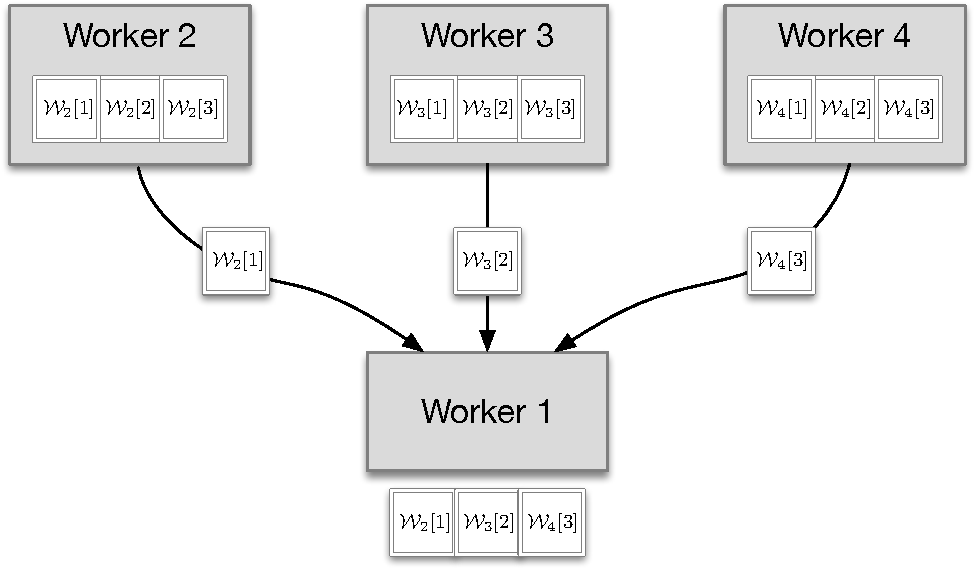
\includegraphics[width=0.3\textwidth]{pics/seg_pull.pdf}
%\caption{Segmented Pulling}
%\label{Fig: seg-pull}
%\end{figure}


\subsubsection{Model Replica}

% Like other gossip-based approaches, we use random partial aggregation as an approximation of the global aggregation. But if the number of the participating workers is too big, which could be common in a federated learning context, there might be huge deviation in such approximation if the worker aggregates local model with only one external model as there are many of them. 
% 

In traditional distributed ML scenario within the datacenter, the gossip-based solutions can choose only one other worker for aggregation but still achieve excellent convergence, because the workers ``gossip" with each other frequently such that the update of each worker are propagated through the whole network before they become too stale\cite{daily2018gossipgrad:}. However, for communication efficient FL systems, the staleness of the model updates is hard to bound as the models are trained separately for up to a few epochs. 
 

Thus as a compromise, we set a hyper-parameter \textit{Model Replica} $R$ which represents the number of the mixed model gathered by segmented pulling. To rebuild $R$ mixed models, the worker will pull $S \times R$ segments from peers. Thus increasing the value of $R$ means more segments have to be transferred through the network, which may cause bandwidth overhead. But this is necessary to accelerate the propagation and ensure the model quality. Since there is no centralized server bottleneck, the model training speed could still be faster even with extra transmission.


\subsubsection{Bandwidth-Aware Gossip Aggregation}
\begin{algorithm}[!t]

\caption{Bandwidth-Aware Combo (BACombo)}

\renewcommand{\algorithmicrequire}{\textbf{Input:}}
\renewcommand{\algorithmicensure}{\textbf{Output:}}
\SetKwFunction{SP}{{SegPulling}}
\SetKwFunction{SA}{{SegAggregation}}


\begin{algorithmic}[1]
\REQUIRE $K, T, \eta, E, \widetilde{w}_0, N, S, \epsilon $

\STATE \textbf{Each worker $i$ executes:}
\STATE $ B \leftarrow \mathbf{0} $

\FOR {$t = 0, ...,T-1$}
    \STATE $r_t \leftarrow Random()$ 
    \STATE updates ${ w}_{t}$ for $E$ epoches of SGD on $F_i$  with step size $\eta$ to obtain ${ w}_{t+1}$
    \IF{ $r_t < \epsilon $}{
        \STATE %$ \{{w}_{t,k}^\prime\}, J, \{D_j\} \leftarrow $ 
        \SP{$Random(),K, N,i$}
        \STATE update $B$ based on the \textbf{BandwidthPrediction}$(J)$}
    \ELSE {
        \STATE %$ \{{w}_{t,k}^\prime\}, J, \{D_j\} \leftarrow $ 
        \SP{$Greedy(),K, N,i$}
    } 
    \ENDIF
    \STATE $\widetilde{{w}}_{t+1} \leftarrow$ \textbf{SegAggregation} $(\{{w}_{t,k}^\prime\},{{w}}_{t+1},J ,\{D_j\})$
\ENDFOR
\item[]

\STATE \SP{$k,w_{t}$}//Run on worker $k$
{
    \STATE \quad worker $k$ updates $w_t$ for $E$ epoches of SGD on $F_k$ \\ \quad with step size $\eta$ to obtain $w_{t+1}$
\RETURN $w_{t+1}$ 
}

\item[]

\STATE \SA{$k,w_{t}$}//Run on worker $k$
{
    \STATE \quad worker $k$ updates $w_t$ for $E$ epoches of SGD on $F_k$ \\ \quad with step size $\eta$ to obtain $w_{t+1}$
\RETURN $w_{t+1}$ 
}

\end{algorithmic}	\label{BACombo} 
\end{algorithm}

            % \STATE worker selects a subset $S_{t}$ of S segments at random (each segments $s$ is chosen from  with probability $p_s$)
            
        %             \FOR {$ k = 1, ..., K$}
            
        % \ENDFOR
                % \STATE worker selects a subset $S_{t, s, r}$ of  workers at random (each worker $k$ is chosen with probability $p_k$)
%The \sys worker updates its local model using multiple "local models" from peers, each local model is a composition of model segments from different peers, we call the composition \textit{Model Replica}.

%
%the workers pull their local model to peers instead of center server.  
%
%When a worker $i$ finishes the local training and seeking to do the model aggregation, it reports its status to the index server. And then the server randomly samples a subset $K_i$ from all the participating workers as the aggregation candidates of worker $i$ and send the information about $K_i$ to worker $i$. To control the training progress, the workers of $K_i$ should have the same training iterations. When worker $i$ receives the candidate list $K_i$, it proactively fetches the model from the candidate workers, do the aggregation and then continue training on the local dataset. We use an index server to track the information of workers instead of storing peer information on the workers directly because with the growth of the workers and the variation of the network environment, the synchronization overhead can be very huge.
%
% By increasing the initiative of the workers, the bottleneck of server is removed because the communication of the server is trivial and the model parameters, which is the heavy part, are transferred among $n(n-1)$ links of all the workers.

%\subsection{Worker Segmented Transfer and Aggregation}
%After ... , the worker will ... transfer and aggregation...
% 一句话描述他们要干什么


%The idea of pulling model parameters from peers is quite similar with the Gossip-based protocols in which the workers randomly push the models to others. So they are facing the same challenge that the overall transmission quantity is increased for a single worker. In the traditional parameter server architecture, in one global iteration, the worker only has to send and receive for one time. But with the gossip methods, each worker is expected to send and receive for $|K_i|$ times in one iteration. 

%
%As shows in Figure \ref{Fig: Segment sub.1}, when the worker $i$ receives the manifest of $K_i$ candidate worker list from index server.  if the model are break in to $S$ and the replica is set to be $R$. For each segment $l$, worker $i$ selectively choose a worker $N_l$ from the candidate list, and then fetch the corresponding segment from worker $N_l$ which we denote as $\mathcal{W}[l;N_l]$. Note that this step can be parallelized, and to simplify, we use a uniform random sampling method to choose the peers. 

%With the segmented transfer method, worker $i$ receives model information from multiple peers with the transfer size equal to one model. Thus in the aggregation phase, the aggregation result can be affected by more datasets and this could help to increase the generality of the model. But if the number of the participating workers is too big, which could be common in a federated learning context, the segments can only cover few workers. Increasing the number of segments might help but an extremely small segment size could lead to over-mottled parameters. Thus as a compromise, we set a hyper-parameter $R(eplica)$ which means the number of the mixed model rebuilt by Segmented Transfer. 
%
%Another shining point of segmented transfer is privacy preserving. The complete model parameter or gradient set has the potential to leak private data information under attack. Instead of pulling the whole model from peers, \sys only collects a random subset of the parameters, which helps to preserve the data privacy. 

\begin{figure}[H]
\centering 
\subfigure[Segmented Pulling]{
\label{Fig: Segment sub.1}
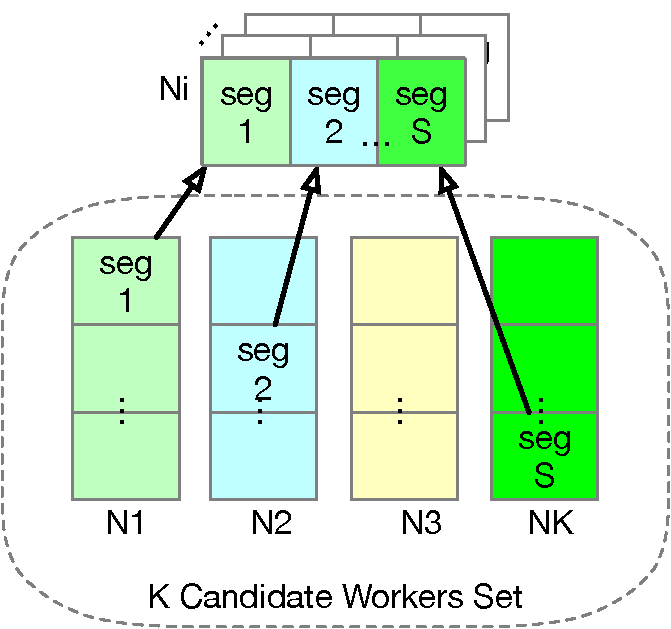
\includegraphics[width=0.2\textwidth]{pics/transfer.pdf}}
\subfigure[Segmented Aggregation]{
\label{Fig: Segment sub.2}
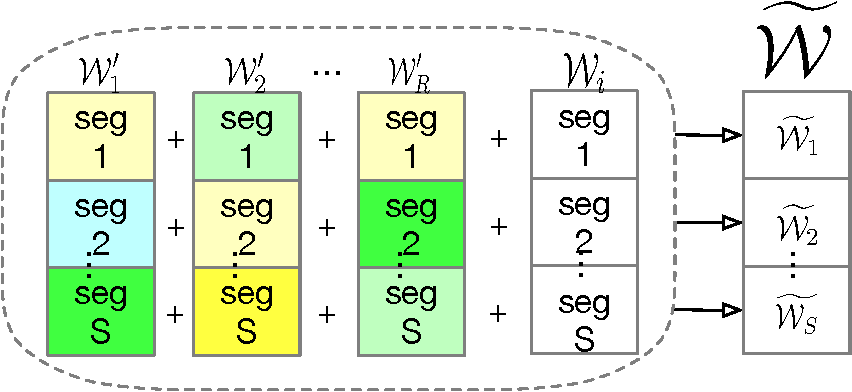
\includegraphics[width=0.225\textwidth]{pics/aggregation.pdf}}
\caption{Segmented Gossip Aggregation}
\label{Fig: Segmented schema}
\end{figure}

\subsubsection{Segmented Aggregation}
%When it fetches all the segments back, a new mixed model can be rebuilt as:
%\begin{equation}
%    \mathcal{W}^\prime = \bigcup_{l = 1}^{S} \mathcal{W}[l;N_l] \label{eq:seg_union}
%\end{equation}
Typically the model aggregation uses weighted averaging of the received model parameters with the worker's dataset size as weight. But in segmented gossip aggregation, the mixed models are patched together from different workers, so it is hard to set a reasonable weight for the mixed model as a whole. For such case, we use a segment-wise model aggregation. 

 Assume the worker $i$ has fetched all the segments and rebuilt $R$ mixed models which we represent as $\mathcal{W}^\prime_1,\mathcal{W}^\prime_2, \dots ,\mathcal{W}^\prime_R$. Then for each segment $l$, we have $R$ mixed models and one local model to aggregate. Let $P_l$ denote the set of the workers which provide the segment $l$ (worker $i$ itself is contained too) and $|D_j|$ denote the dataset size of worker $j$, then we can aggregate segment $l$ by:
 
 \begin{equation}
 \label{eq:seg_agg}
     \widetilde{\mathcal{W}}[l] = \frac{\sum_{j\in P_l}|D_j|\mathcal{W}_j[l]}{\sum_{j\in P_l}|D_j|}
 \end{equation}

Combine all the aggregated segments, and we can rebuild the final aggregation result by 
\begin{equation}
    \mathcal{W} = (\widetilde{\mathcal{W}}[1],\widetilde{\mathcal{W}}[2],\dots,\widetilde{\mathcal{W}}[S])
\end{equation}
And then the worker can continue its training until next aggregation phase comes.
 

\section{\sys Design}
In this section, we introduce \sys, a decentralized federated learning system based on segmented gossip aggregation. We firstly present the implementation details of \sys, then discuss how it handles the dynamic nature of FL workers, and finally, we give a brief analysis of the convergence of \sys.

\subsection{Implementation Details}
As a decentralized FL system, we focus on the design of the workers as the participation of the centralized server is not required during the training. However, it's important to notice that before the training starts, the server has to initialize the model parameters of each worker with the same value otherwise the training may fail to converge. 

A \sys worker follows a stateful training process as illustrated by the numbered steps in Fig.\ref{Fig: worker-arch}. At each iteration, the workers (1) update the model with local dataset and meanwhile, (2) send the segment pulling requests to other workers, once the update is finished, they (3) send the segments to the requestors as a response of the pulling requests and when all the pulling requests are satisfied, the workers (4) aggregate the model segments and start next iteration. Next, we describe the implementation details of these steps.

\noindent{\bf (1) Local Update.} The learning process starts with the worker updating the model with the local dataset. The worker takes the aggregation result of the last iteration as the input model and updates it using stochastic gradient descent(SGD) with the local data. To reduce the communication cost, the local update may contain multiple SGD rounds before the communication with other workers. We denote the communication interval or the number of SGD rounds as $\tau$, which, in typical FL systems, could be up to a few epochs.

\noindent{\bf (2) Segments Pulling.} The workers firstly decide how to partition the model. They don't have to follow the same partition rule, but for simplicity, we assume they partition the model into $S$ segments in the same way. For each segment, the worker has to select $R$ peers and sends the \emph{pulling request}, which contains a segment description and a unique identifier of the worker to indicate which part of the model is to be sent and whom it suppose to be sent to. 

Each worker has to send $S\times R$ segment pulling requests to the other workers, and \sys tries to distribute these requests evenly among all the workers to engage more links and balance the transmission workload. Thus for each request, the target worker is randomly selected from all the other workers without replacement until there is no option left, which means when $S\times R \leq n$, all the segments come from different workers. Note that for each iteration, the pulling requests can be sent even before the local update starts; in this way, the target workers can send the segments immediately when the local model is ready.

\noindent{\bf (3) Segments Sending.} The sending procedure is a twin action of the segments pulling. When the worker finishes the local update, it is ready to send its update result to others. Rather than actively pushing the model, the worker only dispatches the model segments according to the received pulling requests.

\noindent{\bf (4) Model Aggregation.} While the worker is providing the model segments to others, it is also receiving the segments it has requested previously. The model aggregation phase is blocked until all the pulling requests are satisfied, then the worker aggregates the external model segments with the local model using \eqref{eq:seg_agg} and put the aggregated segments together to rebuild the model. With the aggregation result, the worker gets back to the first step and starts the next training iteration.


\begin{figure}[H]
\centering 
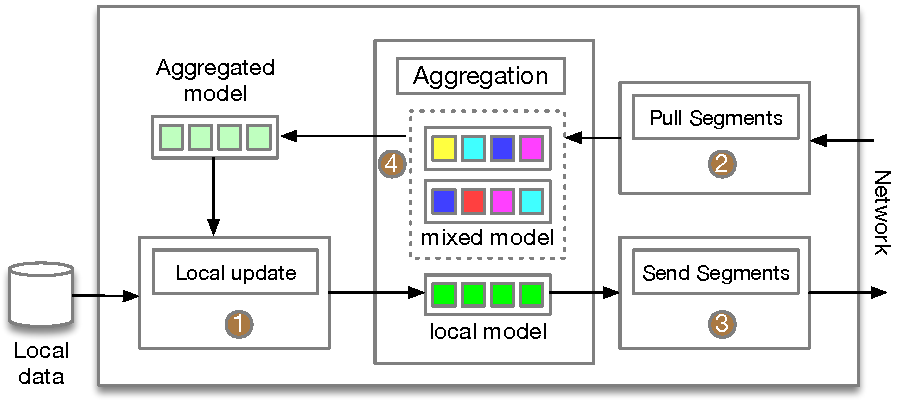
\includegraphics[width=0.49\textwidth]{pics/worker_arch.pdf}
\caption{The architecture of \sys workers}
\label{Fig: worker-arch}
\end{figure}



\subsection{Dynamic Workers}
In the context of federated learning, the participating workers are more likely to be mobile phones and embedded devices, which are often not connected to a power supply and stable network. Thus the workers in FL system are highly dynamic and unstable, and they can join and exit the federation at any time. 

Traditional distributed systems adopt the heartbeat packet and time threshold to check the status of the workers. However, these methods are not applicable with the FL system for the next two reasons: 1) The server has to maintain the heartbeat connection with all the participating workers which limits the scalability of the system. 2) The computation times of each worker vary significantly due to the difference in the computing devices and network environment.

Fortunately, the design of \sys allows us to solve this problem decently. If the worker exits accidentally, the pulling requests it sends to other workers can be canceled immediately when the target workers find it unreachable. For those workers who have requested segments from the offline worker, they can monitor the status of the target workers, and once they see the connection with the target worker is lost, they can mark it as offline, resend the request to another worker and stop pulling from the offline worker. If it is a false report due to the network fluctuation or the offline worker comes back, the offline flag can be removed as long as the communication is reestablished. 

The participation of a new worker is relatively easy to handle. When a new worker comes to the federation, it first requests a worker list either from a server or an old worker. Then it pulls the segments and aggregates them as normal only without its own local model. With the aggregation result, it can start the training with its local dataset. When it sends the pulling requests to the target workers, the target worker adds the newcomer to the worker list. Since the new worker sends the pull requests to many workers in a single iteration, its existence will be quickly noticed by all other workers, and then the new worker successfully joins the federation.




\subsection{Convergence Analysis}

\newtheorem{theorem}{\bf Theorem}
\newtheorem{define}{\bf Definition}
\newtheorem{assumption}{\bf Assumption}

Generally, the deep learning uses the gradient descent algorithms to find the model parameters that minimize a user-defined loss function which we denote it as $F(\mathcal{W})$. For the loss function, we make the following assumptions.

\begin{assumption}
{\bf (Loss function)} $F(\mathcal{W})$ is a convex function with bounded second derivative such that
\begin{equation}
    \mu \leq ||\nabla^2F(\mathcal{W})|| \leq L
\end{equation}
\end{assumption}

In a centralized learning system, the model parameters are updated with the gradient $\nabla F(\mathcal{W})$ calculated from the whole dataset. But with the federated settings, the worker $i$ updates the model with the gradient of a subset of data and we denote it as $\nabla F_i(\mathcal{W})$. To capture the divergence of these two gradients, we make the next definition.

\begin{define}
    {\bf (Gradient Divergence)} For any worker $i$ and model parameter $\mathcal{W}$, We define $\delta$ as the upper bound of the divergence between local and global gradients.
    \begin{equation}
      || \nabla F_i(\mathcal{W}) - \nabla F(\mathcal{W})|| \leq \delta
    \end{equation}
\end{define}

For a worker $i$ in our proposed system, at iteration $t$, the local model parameter $\mathcal{W}_{t,i}$ is an aggregation result of the local model and a few mixed models rebuilt from segments. As a contrast, we denote $\mathcal{W}_{t}$ as the aggregation result of all the nodes, which is the output of $FedAvg$ algorithm. Like the gradient divergence, we define aggregation divergence to measure the aggregation result.

\begin{define}
    {\bf (Aggregation Divergence)} For any worker $i$ at iteration $t$, we define $\rho$ as the upper bound of the divergence between partial and global aggregation.
    \begin{equation}
      || \mathcal{W}_{t,i} - \mathcal{W}_{t}|| \leq \rho
    \end{equation}
\end{define}

With the above assumption and definitions, we can present the convergence result of \sys. 

\begin{theorem}
\label{trm:converge}
    Let $\mathcal{W}^*$ denote the global optimum and $\mathcal{W}_0$ denote the initial model parameters, worker $i$ performs gradient descent on local dataset for $\tau$ times with learning rate $\alpha \leq \frac{1}{L}$ and then pull the segments to aggregate, the aggregation result is $\mathcal{W}_{t,i}$, the convergence upper bound of \sys is given by
    \begin{equation}
            ||\mathcal{W}_{t,i}-\mathcal{W}^*|| \leq \theta^{t\tau} ||\mathcal{W}_{0}-\mathcal{W}^*|| + (1-\theta^{t\tau})[\frac{\rho}{1-\theta^\tau} + \frac{\alpha \delta}{1-\theta}]
    \end{equation}
    where $\theta = 1-\alpha \mu$.
\end{theorem}
\newenvironment{ProofSketch}{%
  \renewcommand{\proofname}{\bf Proof Sketch}\proof}{\endproof}
  
%\begin{ProofSketch}
%This is proof
%\end{ProofSketch}

%Note that this bound is characteristic of stochastic gradient descent bounds that it converges to within a noise ball around the optimum rather than approaching it. The gap between the output and optimum comes from two part: the gradient divergence $\delta$ and the aggregation divergence $\rho$. The gradient divergence is related to the data distribution of each worker which is not alterable. According to the above inequality, the influence of $\rho$ is exacerbated when the communication interval $\tau$ increases. The aggregation divergence can be ameliorated by aggregating more models from other workers. This explains why we set a hyper-parameter $R$ to control the model replicas received from others.

Note that this bound is characteristic of stochastic gradient descent bounds that it converges to within a noise ball around the optimum rather than approaching it. The gap between the output and optimum comes from two part: the gradient divergence $\delta$ and the aggregation divergence $\rho$. The gradient divergence is related to the data distribution of each worker, which is the inherent drawback of the FL system.

According to the above inequality, the influence of $\rho$ is exacerbated when the communication interval $\tau$ increases. The aggregation divergence can be ameliorated by aggregating more models from other workers. This explains why we set a hyper-parameter $R$ to control the model replicas received from others. If we let $R=n-1$, the worker aggregates all the external models and the model divergence decreases to zero. In this situation, \sys degrades to the all-reduce scheme and has the same training result as the centralized way. However, we argue that the value of $R$ could be much smaller but still maintains the training efficiency, which is then validated in the evaluation.



















\begin{algorithm}
    \label{alg:restrict_update}
    \SetAlgoLined
    \SetKwInOut{KIn}{Input}
    \SetKwInOut{KOut}{Output}
    \caption{Restricted local update}
    \KIn{client $k$, global weights $w$, interval $\tau$}
    \KOut{local training result $w^\prime$}
    $w^\prime \leftarrow w$\;
    \For{local iteration $i=1,2,\dots, \tau$}{
        $b \leftarrow$ random batch of training samples\;
        $g \leftarrow$ the gradients of $w^\prime$ on batch $b$\;
        \eIf{$w^\prime$ is overfitted}{
            \textbf{break}\;
        }{
        $w^\prime \leftarrow w^\prime - \mu g$\;
        }
    }
    \Return $w^\prime$
\end{algorithm}


%%\newcommand{\sys}{Combo}

\section{Model Decomposition and Synthesis (MDS)}
%描述过程和具体设计(软件工程详细设计
\subsection{Worker Proactive Pulling}
When a node $i$ finishes the local training and seeking to do the model aggregation, it reports its status to the index server. And then the server randomly samples a subset $K_i$ from all the participating nodes as the aggregation candidates of node $i$ and send the information about $K_i$ to node $i$. To control the training progress, the nodes of $K_i$ should have the same training iterations. When node $i$ receives the candidate list $K_i$, it proactively fetches the model from the candidate nodes, do the aggregation and then continue training on the local dataset. We use an index server to track the information of nodes instead of storing peer information on the nodes directly because with the growth of the nodes and the variation of the network environment, the synchronization overhead can be very huge.

 By increasing the initiative of the nodes, the bottleneck of server is removed because the communication of the server is trivial and the model parameters, which is the heavy part, are transferred among $n(n-1)$ links of all the nodes.

\subsection{Worker Segmented Transfer and Aggregation}
After ... , the worker will ... transfer and aggregation...
% 一句话描述他们要干什么
\sys borrows the idea of ...

The idea of pulling model parameters from peers is quite similar with the Gossip-based protocols in which the nodes randomly push the models to others. So they are facing the same challenge that the overall transmission quantity is increased for a single node. In the traditional parameter server architecture, in one global iteration, the node only has to send and receive for one time. But with the gossip methods, each node is expected to send and receive for $|K_i|$ times in one iteration. 
\subsubsection{Segmented Transfer}
% 描述详细的设计
Let $\mathcal{W}$ denote the model parameters, we break $\mathcal{W}$ into $S$ segments such that:
\begin{equation}
    \begin{split}
        \bigcup_{l = 1}^{S} \mathcal{W}[l] &= \mathcal{W} \\
        \mathcal{W}[l] \cap  \mathcal{W}[m] &= \emptyset \quad \forall l\neq m
    \end{split}
\end{equation}
The segment process doesn't have to be sequential as long as it follows the above requirement, but the segment rule must be clear, that is for any model parameter, you have to know which segment it belongs to. 

When the node $i$ receives the candidate list $K_i$ from index server. For each segment $l$, node $i$ randomly choose a node $N_l$ from the candidate list, and then fetch the corresponding segment from node $N_l$ which we denote as $\mathcal{W}[l;N_l]$. Note that this step can be parallelized. When it fetches all the segments back, a new mixed model can be rebuilt as:
\begin{equation}
    \mathcal{W}^\prime = \bigcup_{l = 1}^{S} \mathcal{W}[l;N_l] \label{eq:seg_union}
\end{equation}

With the segmented transfer method, node $i$ receives model information from multiple peers with the transfer size equal to one model. Thus in the aggregation phase, the aggregation result can be affected by more datasets and this could help to increase the generality of the model. But if the number of the participating nodes is too big, which could be common in a federated learning context, the segments can only cover few nodes. Increasing the number of segments might help but an extremely small segment size could lead to over-mottled parameters. Thus as a compromise, we set a hyper-parameter $R(eplica)$ which means the number of the mixed model rebuilt by Segmented Transfer. 

Another shining point of segmented transfer is privacy preserving. The complete model parameter or gradient set has the potential to leak private data information under attack. Instead of pulling the whole model from peers, \sys only collects a random subset of the parameters, which helps to preserve the data privacy. 


 \begin{figure}[H]
\centering 
\subfigure[Segment Transfer]{
\label{Fig: Segment sub.1}
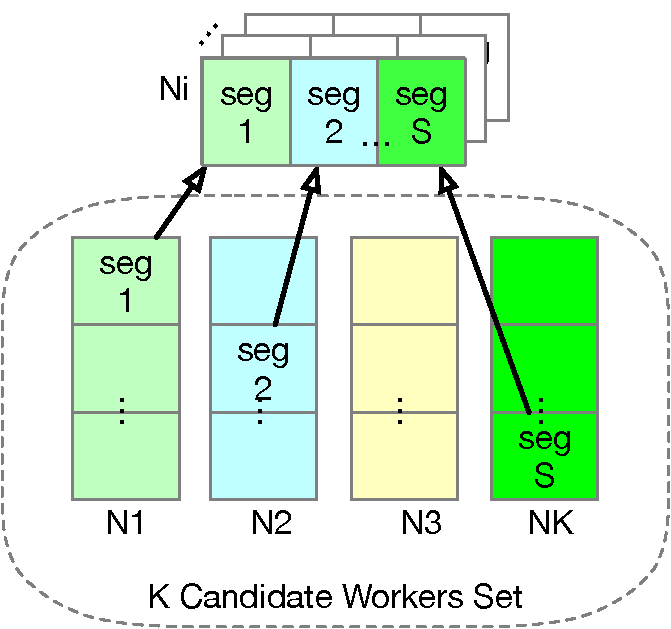
\includegraphics[width=0.225\textwidth]{pics/transfer.pdf}}
\subfigure[Segment Aggregation]{
\label{Fig.Segment sub.2}
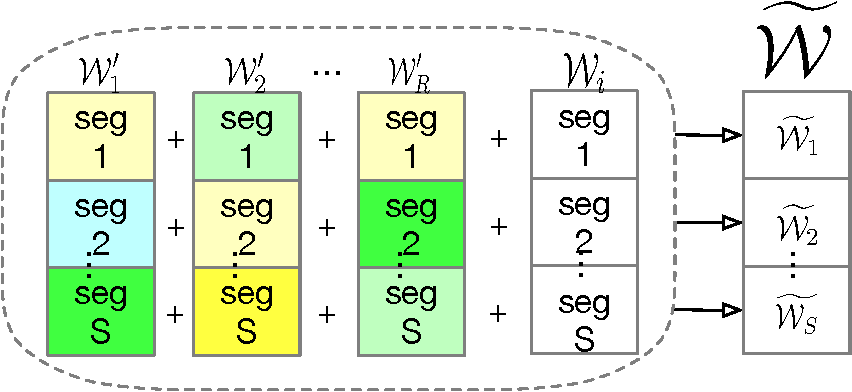
\includegraphics[width=0.225\textwidth]{pics/aggregation.pdf}}
\caption{Segment Transfer and }
\label{Fig: Segment}
\end{figure}

\subsubsection{Segmented Aggregation}
Typically the model aggregation uses weighted mean of the model parameters with the node's dataset size as weight. But in \sys, the mixed models are patched together so it is hard to set a reasonable weight for the mixed model as a whole. For such case, we use a segment-wise model aggregation in \sys.

 Assume the node $i$ has has fetched all the segments and rebuilt $R$ mixed models which we represent as $\mathcal{W}^\prime_1,\mathcal{W}^\prime_2, \dots ,\mathcal{W}^\prime_R$. Let $\mathcal{W}$ denote the model parameters of node $i$. First, we break $\mathcal{W}$ to $S$ segments using the same rule as the segmented transfer. Then for each segment $l$, we have $R$ mixed models and 1 local model to aggregate. Let $P_l$ denote the set of the nodes which provide the segment $l$(node $i$ is contained too) and $|D_j|$ denote the dataset size of node $j$, then we can aggregate segments $l$ by:
 \begin{equation}
     \widetilde{\mathcal{W}}[l] = \frac{\sum_{j\in P_l}|D_j|\mathcal{W}[l;j]}{\sum_{j\in P_l}|D_j|}
 \end{equation}

With all the aggregated segments $\widetilde{\mathcal{W}}[l]$, we can rebuild the final result by using \eqref{eq:seg_union}. And then the node can continue its training until next aggregation phase comes.

\subsection{Server Dynamic Configuration}

\subsubsection{Available Worker Updates}


\subsubsection{Fault Tolerence}
In the context of federated learning, the participating nodes are more likely to be mobile phones and embedded devices, which are often not connected to a power supply and stable network. To ensure the availability of the devices, traditional distributed systems adopt the heartbeat packet and time threshold to determine the status of the nodes. However, these methods are not applicable with federated learning for next two reasons: 1) The server has to maintain the heartbeat connection with all the participating nodes which limits the scalability of the system. 2) The computation times of each nodes vary greatly due to the difference of the computing devices and network environment.

Fortunately, the design of \sys gives us an opportunity to solve this problem decently. In the normal situation, when a node comes to the federation, it just has to register itself on the index server, pull the newest model segments to rebuild a model as its own, and then it's in. When it quits, it should wipe out its record at index server so other nodes won't request its model.

And the interesting thing is that when the node exits accidentally, it doesn't affect the federation at all. The node won't be noticed if no one requests model from this node. And if a node does randomly chooses this absent node as its target and fails to connect, it just has to select another node and report the absence to the server. Then the server know it's time to stop providing this absent node as candidate and delete the record. And if it is a false report due to the network connection, the index can be quickly rebuilt as long as the communication between the absent node and the index server reestablished. 
\section{Performance Evaluation}

%The evaluation of \sys can be divided into two parts. We develop a virtual network environment with Mininet which is able to build complex network topology and run real data transmission by virtualizing multiple kernels. The bandwidth is limited to simulate the real WAN environment and we program the virtual kernels to train and communicate according to the protocols of federated averaging algorithm and \sys. Note that in the network simulation, the kernel performs pseudo-training which only consumes time but trains nothing. On the other hand, we perform the training process on a single machine with 4x NVIDIA GTX 1080 Ti graphic cards. The training process is logically identical with the real distributed systems only but it executes the training of each node sequentially. Some details are as follows:

\subsection{Setup}

We conduct simulation experiments to evaluate our design. The evaluation can be divided into two parts. First, the stateful and synchronous nature of \sys allows us to simulate the training process sequentially, while logically, the training result is the same as the parallelized way. The training traces of each worker are then recorded, which contains the validation accuracies, training iterations, and corresponding synchronization partners. Second, we simulate the network topology and feed it with the training traces to estimate the training time. The specific settings are listed as follows:

$\triangleright$ \textit{Training settings.} We train a CNN model on CIFAR-10 dataset to evaluate the training ability of \sys. The dataset consists of  50,000 images for training and 10,000 for validation. The training data are randomly distributed among the workers without overlapping, and the validation data are shared among every worker. The CNN model is adopted from \cite{McMahan2017FL}, which is considered to be suitable for CIFAR-10 dataset. 

The models are trained on each worker using SGD algorithm with the same hyper-parameters, that a learning rate of 0.1 and a batch size of 128. The synchronization interval is set to 40, which means every worker perform SGD updates on the local model for 40 times before it communicates with others.

$\triangleright$ \textit{Network settings.} We simulate a fully connected network topology among the workers. The maximum bandwidth limit of each worker is set to be 100Mbps. Moreover, to simulate the bottleneck of WAN, we set 10Mbps as the available bandwidth between two workers.

$\triangleright$ \textit{Comparison settings.} We compare \sys and (1) traditional federated learning system with a \emph{centralized} parameter server and (2) naive \emph{gossip} approach without segmentation. To make them comparable, they are all simulated within the same network topology, and for the centralized system, we randomly choose one worker to play the role of parameter server.

The communication behavior of \sys is controlled by two parameters: \emph{model segments} as $S$ and \emph{model replica} as $R$. In our following experiments, we set $S=10$ and $R=2$ by default, that is in the synchronization phase, the model is partitioned into ten segments, and for each segment, the worker requests two replicas from other workers. The gossip approach is the special case of \sys when $S=1$, and it shares the same value of $R$ with \sys.


$\triangleright$ \textit{Performance Metrics.} The learning performance is measured by the convergence speed. We record the top-1 validation accuracies of the aggregated models at each round and then align the accuracies to the corresponding times. The time is acquired from our network simulator where the local update time is referenced from the real machine time of training with a GTX 1080 Ti graphics card, and the communication time is calculated according to the bandwidth limitations.


\subsection{Experiment Result}

We first evaluate the convergence speed and scalability of \sys in comparison to the other approaches, then we explore the advantages and disadvantages of the design of model segments and replicas and how they affect the training performance.

\subsubsection{Convergence Speed}

We present the whole training process over time, as illustrated in Fig.\ref{Fig: time_acc_30}, \sys exhibits an apparent speedup in the convergence without affecting the final validation accuracy. We also explore the scalability of these three methods by comparing the training time needed to reach a predefined accuracy goal with varying number of workers among 20, 30, and 40. According to Fig.\ref{Fig: time_acc_30}, the model reaches convergence around 82\% validation accuracy. Since the aim is not achieving the best accuracy and practically speaking, it is not worthy of spending too much time for only 1\% or 2\% accuracy gain. Thus we set 80\% as the accuracy goal. 

As illustrated in Fig.\ref{Fig: scale_time}, \sys requires the least training time to reach the given accuracy within all three cases and compared with the centralized system, the speedup of \sys increases from $2.25\times$ to $3.01\times$ with the expansion of scale. This phenomenon indicates that the decentralized federated learning is more scalable than the centralized way. Additionally, both as the decentralized approaches, \sys almost reduces the training time by half compared with the naive gossip solution.

%%%%%%%%%%%%%%%%%%%%%%%%%%%%%
\begin{figure*}[htbp]

\begin{minipage}[t]{0.32\textwidth}%%\centering
\subfigure[Convergence with 30 workers]{
\label{Fig: time_acc_30}
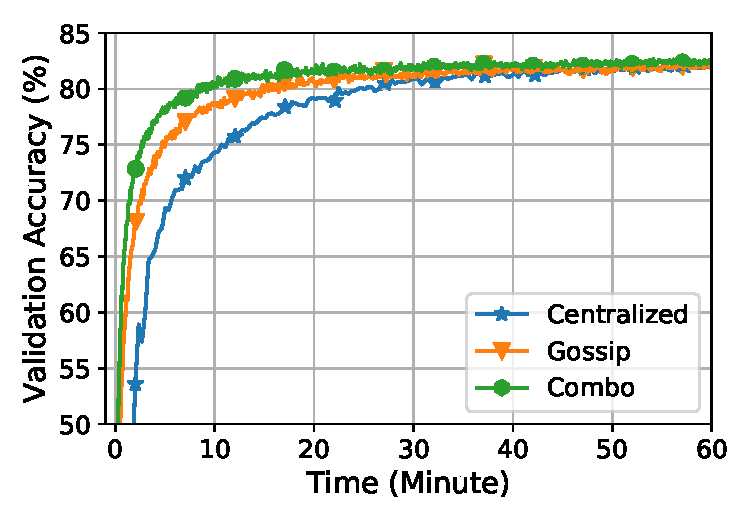
\includegraphics[width=0.9\textwidth]{pics/time_acc_30_refill.pdf}}
\\
\subfigure[Time to reach 80\% accuracy]{
\label{Fig: scale_time}
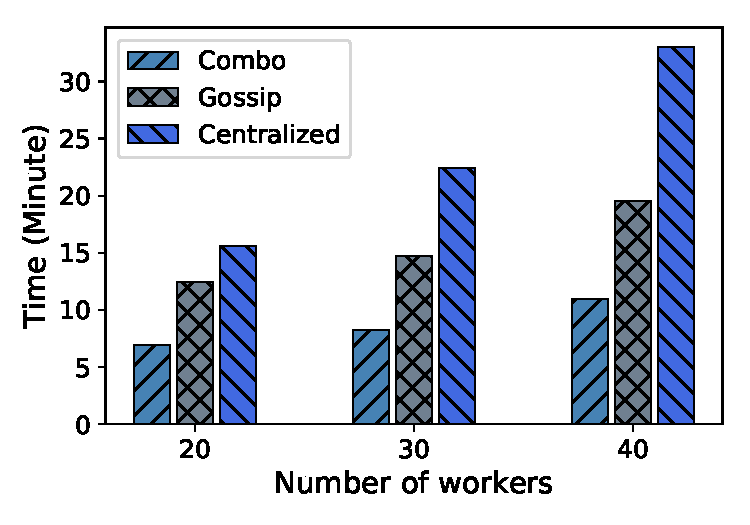
\includegraphics[width=0.9\textwidth]{pics/scale_time_refill.pdf}}

\caption{Convergence speed}
\label{Fig: acc}
\end{minipage}
\begin{minipage}[t]{0.32\linewidth}
\centering 
\subfigure[Convergence with model segments]{
\label{Fig: seg_acc}
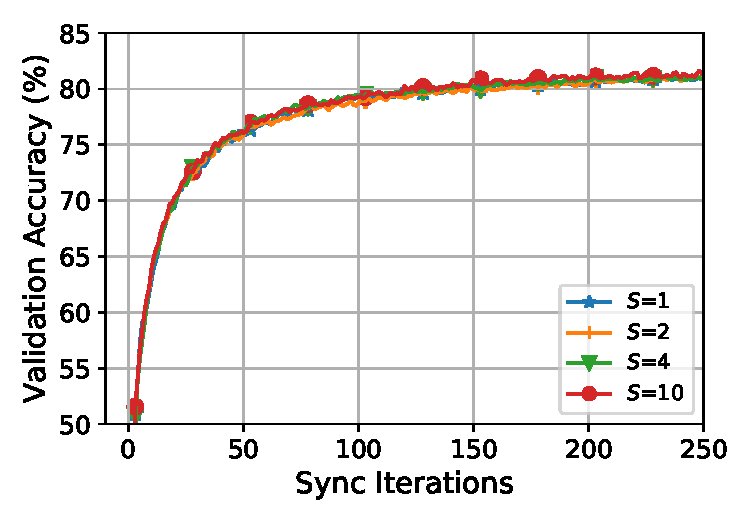
\includegraphics[width=0.9\textwidth]{pics/segment_acc_fill.pdf}}
\\
\subfigure[Sync time comparison]{
\label{Fig: seg_time}
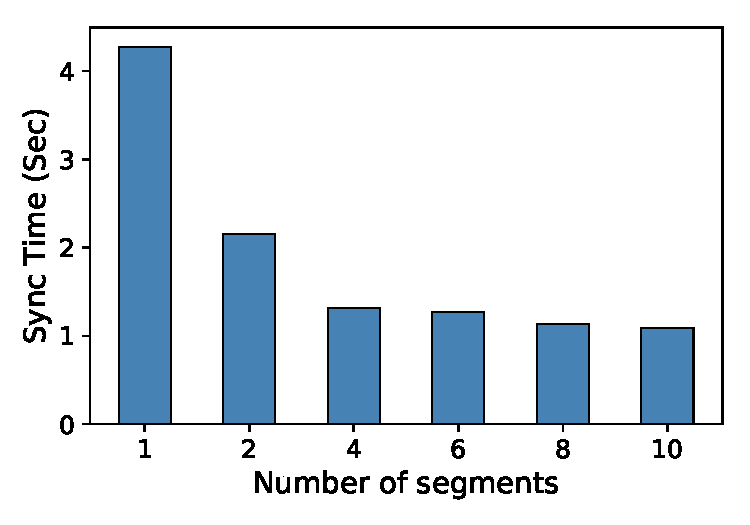
\includegraphics[width=0.9\textwidth]{pics/segment_time.pdf}}
\caption{Benefit of model segments}
\label{Fig: acc}
\end{minipage}
\begin{minipage}[t]{0.32\linewidth}
\centering 
\subfigure[Convergence with model replicas]{
\label{Fig: replica_acc}
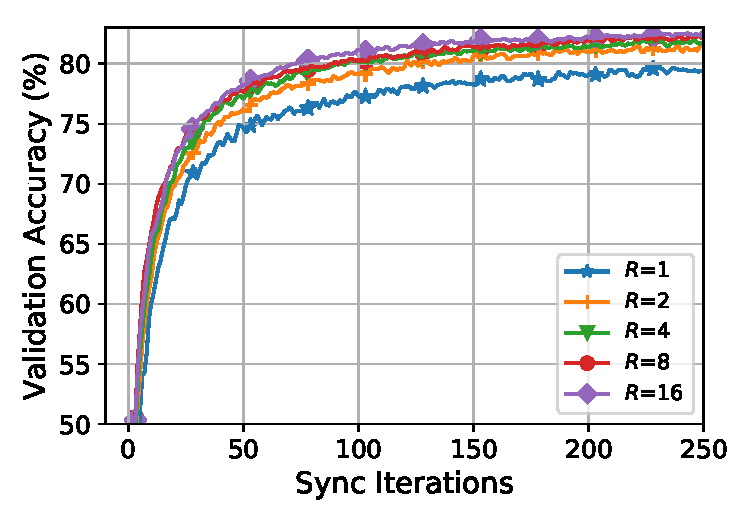
\includegraphics[width=0.9\textwidth]{pics/replica_acc_fill.pdf}}
\\
\subfigure[Time to reach 80\% accuracy]{
\label{Fig: replica_time}
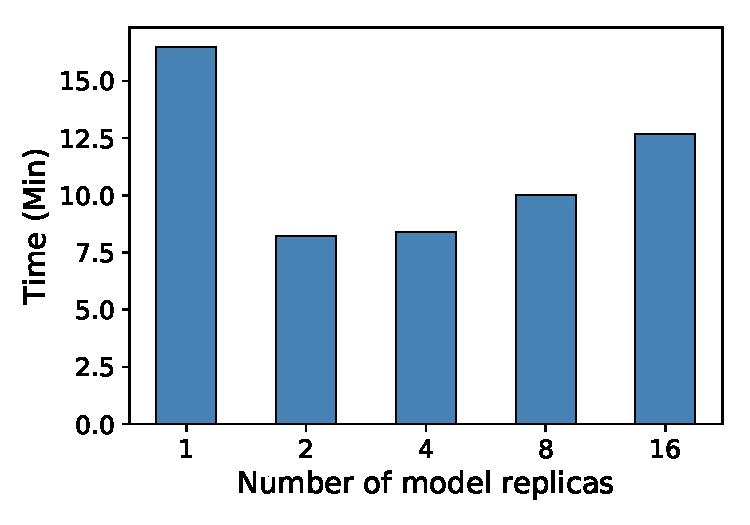
\includegraphics[width=0.9\textwidth]{pics/replica_time}}

\caption{Impact of model replicas}
\label{Fig: acc}
\end{minipage}

\end{figure*}



\subsubsection{Benefit of Model Segments}
The speedup of decentralized approaches comes from the removal of the bottleneck of the centralized server, and the advantage of \sys comes from the benefit of model segments. We train the mode with 30 workers, fix $R=2$ and vary $S$ from 1 to 10 to investigate how model segments affect the training performance.

Compared with the naive gossip solution, \sys aggregates mixed model parameters made up of multiple segments instead of the complete model. A potential concern is that the result may suffer degradation as the aggregation target is mottled and loses integrality. However, Fig.\ref{Fig: seg_acc} shows that the accuracy of the aggregated results at each synchronization iterations is not affected by the model segments at all. Partitioning the model into ten segments($S=10$) has the same convergence trend as that without partition.

While the model segments don't affect the accuracy at each iteration, the synchronization time is significantly reduced. As illustrated in Fig.\ref{Fig: seg_time}, by simply splitting the model parameters into two segments can reduce the synchronization time by half. This is because when $S=2$, the original transmission quantity is divided into two parts and fed into $2\times$ more links. When the bandwidth is not exhausted, the sending and receiving time can be reduced almost proportionally. However, when $S\geq 6$, the bandwidth is already fully exploited, increasing the number of segments will not improve the time consumption then.


\subsubsection{Impact of Model Replicas}

Next, we evaluate the impact of model replica, which controls the overall information quantity that the workers send and receive at each synchronization iterations. Similar to the previous settings, we fix $S=10$ and vary $R$ from 1 to 16.

As we discussed in the convergence analysis of \sys, the more information a worker receives, the better aggregation result it will get. When the worker receives all the model replicas from other peers, \sys becomes the All-reduce structure and achieves the same training result as the centralized approach. The analysis is validated by Fig.\ref{Fig: replica_acc} that with the increase of the number of model replicas, the accuracy of each iteration becomes better. However, the improvement is not unlimited. We can see that there is no significant gap between $R=8$ and $16$ in the convergence trend and result. This reflects the redundancy of All-reduce structure that the worker doesn't have to collect all the external models to train a high-quality model.

However, as the bandwidth of worker is fully utilized with model segments, increasing $R$ leads to the proportional growth of the transmission workload. Thus there exists a tradeoff, a larger $R$ increases the convergence rate on synchronization iterations but also the synchronization time. We compare the training time needed to reach 80\% validation accuracy with different $R$ as shown in Fig.\ref{Fig: replica_time}. Increasing $R=1$ to $2$ leads to a rapid reduction of the required training time as it drastically reduces the iterations needed to achieve target accuracy goal, which is also illustrated in Fig.\ref{Fig: replica_acc}. However, if we continue to increase $R$, the growth of the training time exceeds the reduction of the iterations and slows down the convergence speed.














\section{Conclusion}
One of the most challenging problem of federated learning is the poor network connection as the workers are geo-distributed and connected with slow WAN. To avoid the drawback of high possibility network congestion in centralized parameter sever architecture, which is adopted in today's FL systems, we explore the possibility of decentralized FL solution, called \sys. Taking the insight that the peer-to-peer bandwidth is much smaller than the worker's maximum network capacity, \sys could fully utilize the bandwidth by saturating the network with segmented gossip aggregation. The experiments show that \sys significantly reduces the training time and remains good convergence performance.
%but still has good convergence.

%\section{Introduction}
%
%The {\it IJCAI--19 Proceedings} will be printed from electronic
%manuscripts submitted by the authors. These must be PDF ({\em Portable
%Document Format}) files formatted for 8-1/2$''$ $\times$ 11$''$ paper.
%
%\subsection{Length of Papers}
%
%All paper {\em submissions} must have a maximum of six pages, plus at most one for references. The seventh page cannot contain {\bf anything} other than references.
%
%The length rules may change for final camera-ready versions of accepted papers, and will differ between tracks. Some tracks may include only references in the last page, whereas others allow for any content in all pages. Similarly, some tracks allow you to buy a few extra pages should you want to, whereas others don't.
%
%If your paper is accepted, please carefully read the notifications you receive, and check the proceedings submission information website\footnote{\url{https://proceedings.ijcai.org/info}} to know how many pages you can finally use (and whether there is a special references-only page or not). That website holds the most up-to-date information regarding paper length limits at all times.
%
%\subsection{Word Processing Software}
%
%As detailed below, IJCAI has prepared and made available a set of
%\LaTeX{} macros and a Microsoft Word template for use in formatting
%your paper. If you are using some other word processing software, please follow the format instructions given below and ensure that your final paper looks as much like this sample as possible.
%
%\section{Style and Format}
%
%\LaTeX{} and Word style files that implement these instructions
%can be retrieved electronically. (See Appendix~\ref{stylefiles} for
%instructions on how to obtain these files.)
%
%\subsection{Layout}
%
%Print manuscripts two columns to a page, in the manner in which these
%instructions are printed. The exact dimensions for pages are:
%\begin{itemize}
%\item left and right margins: .75$''$
%\item column width: 3.375$''$
%\item gap between columns: .25$''$
%\item top margin---first page: 1.375$''$
%\item top margin---other pages: .75$''$
%\item bottom margin: 1.25$''$
%\item column height---first page: 6.625$''$
%\item column height---other pages: 9$''$
%\end{itemize}
%
%All measurements assume an 8-1/2$''$ $\times$ 11$''$ page size. For
%A4-size paper, use the given top and left margins, column width,
%height, and gap, and modify the bottom and right margins as necessary.
%
%\subsection{Format of Electronic Manuscript}
%
%For the production of the electronic manuscript, you must use Adobe's
%{\em Portable Document Format} (PDF). A PDF file can be generated, for
%instance, on Unix systems using {\tt ps2pdf} or on Windows systems
%using Adobe's Distiller. There is also a website with free software
%and conversion services: \url{http://www.ps2pdf.com}. For reasons of
%uniformity, use of Adobe's {\em Times Roman} font is strongly suggested. In
%\LaTeX2e{}, this is accomplished by putting
%\begin{quote} 
%\mbox{\tt $\backslash$usepackage\{times\}}
%\end{quote}
%in the preamble.\footnote{You may want also to use the package {\tt
%latexsym}, which defines all symbols known from the old \LaTeX{}
%version.}
%  
%Additionally, it is of utmost importance to specify the American {\bf
%letter} format (corresponding to 8-1/2$''$ $\times$ 11$''$) when
%formatting the paper. When working with {\tt dvips}, for instance, one
%should specify {\tt -t letter}.
%
%\subsection{Title and Author Information}
%
%Center the title on the entire width of the page in a 14-point bold
%font. The title should be capitalized using Title Case. Below it, center author name(s) in  12-point bold font. On the following line(s) place the affiliations, each affiliation on its own line using 12-point regular font. Matching between authors and affiliations can be done using numeric superindices. Optionally, a comma-separated list of email addresses follows the affiliation(s) line(s), using  12-point regular font.
%
%\subsubsection{Blind Review}
%
%In order to make blind reviewing possible, authors must omit their
%names and affiliations when submitting the paper for review. In place
%of names and affiliations, provide a list of content areas. When
%referring to one's own work, use the third person rather than the
%first person. For example, say, ``Previously,
%Gottlob~\shortcite{gottlob:nonmon} has shown that\ldots'', rather
%than, ``In our previous work~\cite{gottlob:nonmon}, we have shown
%that\ldots'' Try to avoid including any information in the body of the
%paper or references that would identify the authors or their
%institutions. Such information can be added to the final camera-ready
%version for publication.
%
%\subsection{Abstract}
%
%Place the abstract at the beginning of the first column 3$''$ from the
%top of the page, unless that does not leave enough room for the title
%and author information. Use a slightly smaller width than in the body
%of the paper. Head the abstract with ``Abstract'' centered above the
%body of the abstract in a 12-point bold font. The body of the abstract
%should be in the same font as the body of the paper.
%
%The abstract should be a concise, one-paragraph summary describing the
%general thesis and conclusion of your paper. A reader should be able
%to learn the purpose of the paper and the reason for its importance
%from the abstract. The abstract should be no more than 200 words long.
%
%\subsection{Text}
%
%The main body of the text immediately follows the abstract. Use
%10-point type in a clear, readable font with 1-point leading (10 on
%11).
%
%Indent when starting a new paragraph, except after major headings.
%
%\subsection{Headings and Sections}
%
%When necessary, headings should be used to separate major sections of
%your paper. (These instructions use many headings to demonstrate their
%appearance; your paper should have fewer headings.). All headings should be capitalized using Title Case.
%
%\subsubsection{Section Headings}
%
%Print section headings in 12-point bold type in the style shown in
%these instructions. Leave a blank space of approximately 10 points
%above and 4 points below section headings.  Number sections with
%arabic numerals.
%
%\subsubsection{Subsection Headings}
%
%Print subsection headings in 11-point bold type. Leave a blank space
%of approximately 8 points above and 3 points below subsection
%headings. Number subsections with the section number and the
%subsection number (in arabic numerals) separated by a
%period.
%
%\subsubsection{Subsubsection Headings}
%
%Print subsubsection headings in 10-point bold type. Leave a blank
%space of approximately 6 points above subsubsection headings. Do not
%number subsubsections.
%
%\paragraph{Titled paragraphs.} You can use titled paragraphs if and 
%only if the title covers exactly one paragraph. Such paragraphs must be
%separated from the preceding content by at least 3pt, and no more than
%6pt. The title must be in 10pt bold font and ended with a period. 
%After that, a 1em horizontal space must follow the title before 
%the paragraph's text.
%
%In \LaTeX{} titled paragraphs must be typeset using
%\begin{quote}
%{\tt \textbackslash{}paragraph\{Title.\} text} .
%\end{quote}
%
%\subsubsection{Acknowledgements}
%
%You may include an unnumbered acknowledgments section, including
%acknowledgments of help from colleagues, financial support, and
%permission to publish. If present, acknowledgements must be in a dedicated,
%unnumbered section appearing after all regular sections but before any
%appendices or references.
%
%Use 
%\begin{quote}
%    {\tt \textbackslash{}section*\{Acknowledgements\}})
%\end{quote}
%to typeset the acknowledgements section in \LaTeX{}.
%
%\subsubsection{Appendices}
%
%Any appendices directly follow the text and look like sections, except
%that they are numbered with capital letters instead of arabic
%numerals. See this document for an example.
%
%\subsubsection{References}
%
%The references section is headed ``References'', printed in the same
%style as a section heading but without a number. A sample list of
%references is given at the end of these instructions. Use a consistent
%format for references. The reference list should not include unpublished
%work.
%
%\subsection{Citations}
%
%Citations within the text should include the author's last name and
%the year of publication, for example~\cite{gottlob:nonmon}.  Append
%lowercase letters to the year in cases of ambiguity.  Treat multiple
%authors as in the following examples:~\cite{abelson-et-al:scheme}
%or~\cite{bgf:Lixto} (for more than two authors) and
%\cite{brachman-schmolze:kl-one} (for two authors).  If the author
%portion of a citation is obvious, omit it, e.g.,
%Nebel~\shortcite{nebel:jair-2000}.  Collapse multiple citations as
%follows:~\cite{gls:hypertrees,levesque:functional-foundations}.
%\nocite{abelson-et-al:scheme}
%\nocite{bgf:Lixto}
%\nocite{brachman-schmolze:kl-one}
%\nocite{gottlob:nonmon}
%\nocite{gls:hypertrees}
%\nocite{levesque:functional-foundations}
%\nocite{levesque:belief}
%\nocite{nebel:jair-2000}
%
%\subsection{Footnotes}
%
%Place footnotes at the bottom of the page in a 9-point font.  Refer to
%them with superscript numbers.\footnote{This is how your footnotes
%should appear.} Separate them from the text by a short
%line.\footnote{Note the line separating these footnotes from the
%text.} Avoid footnotes as much as possible; they interrupt the flow of
%the text.
%
%\section{Illustrations}
%
%Place all illustrations (figures, drawings, tables, and photographs)
%throughout the paper at the places where they are first discussed,
%rather than at the end of the paper.
%
%They should be floated to the top (preferred) or bottom of the page, 
%unless they are an integral part 
%of your narrative flow. When placed at the bottom or top of
%a page, illustrations may run across both columns, but not when they
%appear inline.
%
%Illustrations must be rendered electronically or scanned and placed
%directly in your document. All illustrations should be understandable when printed in black and
%white, albeit you can use colors to enhance them. Line weights should
%be 1/2-point or thicker. Avoid screens and superimposing type on
%patterns as these effects may not reproduce well.
%
%Number illustrations sequentially. Use references of the following
%form: Figure 1, Table 2, etc. Place illustration numbers and captions
%under illustrations. Leave a margin of 1/4-inch around the area
%covered by the illustration and caption.  Use 9-point type for
%captions, labels, and other text in illustrations. Captions should always appear below the illustration.
%
%\section{Tables}
%
%Tables are considered illustrations containing data. Therefore, they should also appear floated to the top (preferably) or bottom of the page, and with the captions below them.
%
%\begin{table}
%\centering
%\begin{tabular}{lll}
%\hline
%Scenario  & $\delta$ & Runtime \\
%\hline
%Paris       & 0.1s  & 13.65ms     \\
%Paris       & 0.2s  & 0.01ms      \\
%New York    & 0.1s  & 92.50ms     \\
%Singapore   & 0.1s  & 33.33ms     \\
%Singapore   & 0.2s  & 23.01ms     \\
%\hline
%\end{tabular}
%\caption{Latex default table}
%\label{tab:plain}
%\end{table}
%
%\begin{table}
%\centering
%\begin{tabular}{lrr}  
%\toprule
%Scenario  & $\delta$ (s) & Runtime (ms) \\
%\midrule
%Paris       & 0.1  & 13.65      \\
%            & 0.2  & 0.01       \\
%New York    & 0.1  & 92.50      \\
%Singapore   & 0.1  & 33.33      \\
%            & 0.2  & 23.01      \\
%\bottomrule
%\end{tabular}
%\caption{Booktabs table}
%\label{tab:booktabs}
%\end{table}
%
%If you are using \LaTeX, you should use the {\tt booktabs} package, because it produces better tables than the standard ones. Compare Tables \ref{tab:plain} and~\ref{tab:booktabs}. The latter is clearly more readable for three reasons:
%
%\begin{enumerate}
%    \item The styling is better thanks to using the {\tt booktabs} rulers instead of the default ones.
%    \item Numeric columns are right-aligned, making it easier to compare the numbers. Make sure to also right-align the corresponding headers, and to use the same precision for all numbers.
%    \item We avoid unnecessary repetition, both between lines (no need to repeat the scenario name in this case) as well as in the content (units can be shown in the column header).
%\end{enumerate}
%
%\section{Formulas}
%
%IJCAI's two-column format makes it difficult to typeset long formulas. A usual temptation is to reduce the size of the formula by using the {\tt small} or {\tt tiny} sizes. This doesn't work correctly with the current \LaTeX{} versions, breaking the line spacing of the preceding paragraphs and title, as well as the equation number sizes. The following equation demonstrates the effects (notice that this entire paragraph looks badly formatted):
%%
%\begin{tiny}
%\begin{equation}
%    x = \prod_{i=1}^n \sum_{j=1}^n j_i + \prod_{i=1}^n \sum_{j=1}^n i_j + \prod_{i=1}^n \sum_{j=1}^n j_i + \prod_{i=1}^n \sum_{j=1}^n i_j + \prod_{i=1}^n \sum_{j=1}^n j_i
%\end{equation}
%\end{tiny}%
%
%Reducing formula sizes this way is strictly forbidden. We {\bf strongly} recommend authors to split formulas in multiple lines when they don't fit in a single line. This is the easiest approach to typeset those formulas and provides the most readable output%
%%
%\begin{align}
%    x =& \prod_{i=1}^n \sum_{j=1}^n j_i + \prod_{i=1}^n \sum_{j=1}^n i_j + \prod_{i=1}^n \sum_{j=1}^n j_i + \prod_{i=1}^n \sum_{j=1}^n i_j + \nonumber\\
%    + & \prod_{i=1}^n \sum_{j=1}^n j_i
%\end{align}%
%
%If a line is just slightly longer than the column width, you may use the {\tt resizebox} environment on that equation. The result looks better and doesn't interfere with the paragraph's line spacing: %
%\begin{equation}
%\resizebox{.91\linewidth}{!}{$
%    \displaystyle
%    x = \prod_{i=1}^n \sum_{j=1}^n j_i + \prod_{i=1}^n \sum_{j=1}^n i_j + \prod_{i=1}^n \sum_{j=1}^n j_i + \prod_{i=1}^n \sum_{j=1}^n i_j + \prod_{i=1}^n \sum_{j=1}^n j_i
%$}
%\end{equation}%
%
%This last solution may have to be adapted if you use different equation environments, but it can generally be made to work. Please notice that in any case:
%
%\begin{itemize}
%    \item Equation numbers must be in the same font and size than the main text (10pt).
%    \item Your formula's main symbols should not be smaller than {\small small} text (9pt).
%\end{itemize}
%
%For instance, the formula
%%
%\begin{equation}
%    \resizebox{.91\linewidth}{!}{$
%    \displaystyle
%    x = \prod_{i=1}^n \sum_{j=1}^n j_i + \prod_{i=1}^n \sum_{j=1}^n i_j + \prod_{i=1}^n \sum_{j=1}^n j_i + \prod_{i=1}^n \sum_{j=1}^n i_j + \prod_{i=1}^n \sum_{j=1}^n j_i + \prod_{i=1}^n \sum_{j=1}^n i_j
%$}
%\end{equation}
%% 
%would not be acceptable because the text is too small.
%
%\section{Algorithms and Listings}
%
%Algorithms and listings are a special kind of figures. Like all illustrations, they should appear floated to the top (preferably) or bottom of the page. However, their caption should appear in the header, left-justified and enclosed between horizontal lines, as shown in Algorithm~\ref{alg:algorithm}. The algorithm body should be terminated with another horizontal line. It is up to the authors to decide whether to show line numbers or not, how to format comments, etc.
%
%In \LaTeX{} algorithms may be typeset using the {\tt algorithm} and {\tt algorithmic} packages, but you can also use one of the many other packages for the task.  
%
%\begin{algorithm}[tb]
%\caption{Example algorithm}
%\label{alg:algorithm}
%\textbf{Input}: Your algorithm's input\\
%\textbf{Parameter}: Optional list of parameters\\
%\textbf{Output}: Your algorithm's output
%\begin{algorithmic}[1] %[1] enables line numbers
%\STATE Let $t=0$.
%\WHILE{condition}
%\STATE Do some action.
%\IF {conditional}
%\STATE Perform task A.
%\ELSE
%\STATE Perform task B.
%\ENDIF
%\ENDWHILE
%\STATE \textbf{return} solution
%\end{algorithmic}
%\end{algorithm}
%
%\section*{Acknowledgments}
%
%The preparation of these instructions and the \LaTeX{} and Bib\TeX{}
%files that implement them was supported by Schlumberger Palo Alto
%Research, AT\&T Bell Laboratories, and Morgan Kaufmann Publishers.
%Preparation of the Microsoft Word file was supported by IJCAI.  An
%early version of this document was created by Shirley Jowell and Peter
%F. Patel-Schneider.  It was subsequently modified by Jennifer
%Ballentine and Thomas Dean, Bernhard Nebel, Daniel Pagenstecher,
%Kurt Steinkraus, Toby Walsh and Carles Sierra. The current version 
%has been prepared by Marc Pujol-Gonzalez and Francisco Cruz-Mencia.
%
%\appendix
%
%\section{\LaTeX{} and Word Style Files}\label{stylefiles}
%
%The \LaTeX{} and Word style files are available on the IJCAI--19
%website, \url{http://www.ijcai19.org}.
%These style files implement the formatting instructions in this
%document.
%
%The \LaTeX{} files are {\tt ijcai19.sty} and {\tt ijcai19.tex}, and
%the Bib\TeX{} files are {\tt named.bst} and {\tt ijcai19.bib}. The
%\LaTeX{} style file is for version 2e of \LaTeX{}, and the Bib\TeX{}
%style file is for version 0.99c of Bib\TeX{} ({\em not} version
%0.98i). The {\tt ijcai19.sty} style differs from the {\tt
%ijcai18.sty} file used for IJCAI--18.
%
%The Microsoft Word style file consists of a single file, {\tt
%ijcai19.doc}. This template differs from the one used for
%IJCAI--18.
%
%These Microsoft Word and \LaTeX{} files contain the source of the
%present document and may serve as a formatting sample.  
%
%Further information on using these styles for the preparation of
%papers for IJCAI--19 can be obtained by contacting {\tt
%pcchair@ijcai19.org}.

%% The file named.bst is a bibliography style file for BibTeX 0.99c
\bibliographystyle{named}
\bibliography{ijcai19}

\end{document}

